% !TeX root = ../main.tex

\chapter{Resultados e Discussões \label{chap:resultados}}


Com o método de otimização proposto realizamos experimentos de classificação e recuperação de formas pelo conteúdo, para dois descritores, com a base de folhas de plantas Flavia \cite{4458016},  que possui $1907$ imagens de folhas de $32$ espécies. A Figura \ref{fig:bases} ilustra imagens das folhas desta base. Cada exemplar ilustrado foi segmentado e colorido de acordo com a espécie ao qual pertence. Essa base de folhas é amplamente utilizada na validação de trabalhos de reconhecimento automático de espécies de plantas. 

\begin{figure}[!htb]
\caption{\label{fig:bases}Amostras de formas de folhas da base de imagens Flavia.}

\centering
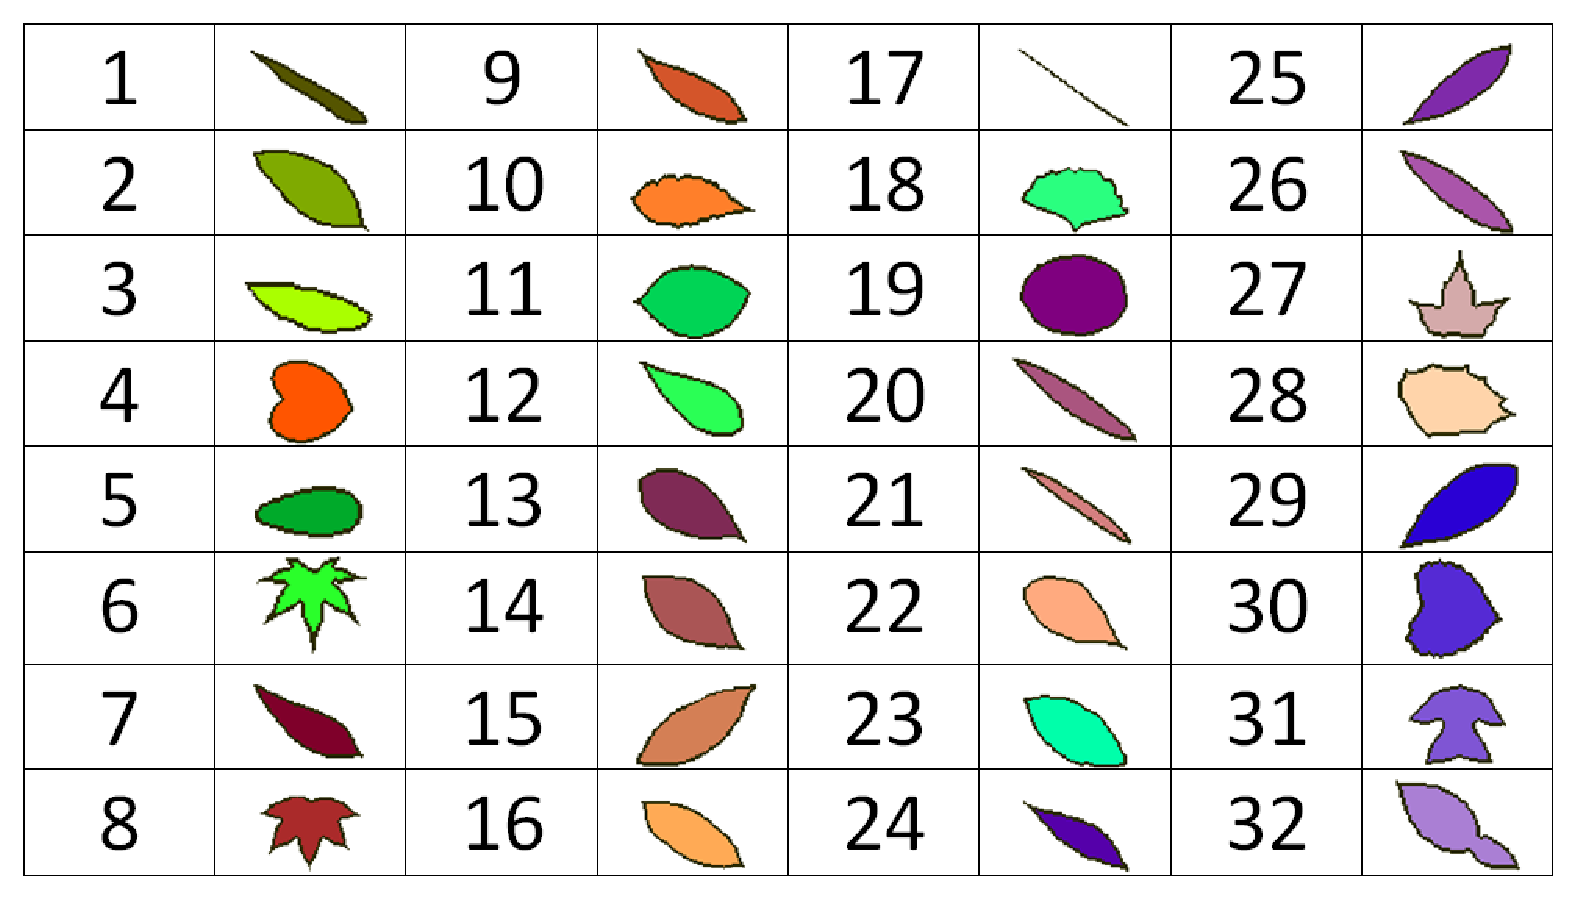
\includegraphics[width=0.5\textwidth]{fig5.eps}
\end{figure}





{\color{blue}

\section{\emph{Classificação de formas e sua relação com  a função objetivo}}
Foram realizados experimentos para comparação dos algoritmos de otimização sob aspecto de convergência. A Figura \ref{fig:converge} ilustra a convergência de cada um dos três algoritmos de otimização para $30$ repetições realizadas em um subconjunto da base de formas de folhas. Os resultados obtidos indicam que a otimização \emph{PSO} requereu um pequeno número de interações para convergir a uma solução ótima quando comparado aos algoritmos \emph{SA} e \emph{DE}. Uma vez que a convergência está relacionada com o número de interações necessárias para se atingir uma solução ótima, poucas interações implicam em uma em exploração deficiente do espaço de busca, ou seja, em convergência prematura \citeonline{Andries:2007}. Nesse caso, o método de otimização apresenta tendência de ficar preso a mínimos locais, encontrando assim soluções sub-ótimas para o problema. Por outro lado, a convergência mais lenta permite ao algoritmo explorar melhor o espaço de busca, aumentando portanto a chance deste convergira um mínimo global, ou seja, uma solução ótima \citeonline{Andries:2007}.
 
Neste contexto, observa-se na Figura \ref{fig:converge}c que o \emph{PSO} encontrou soluções sub-ótimas com maior frequência, alcançando valores médios da função MAD  igual a $0,805 \pm 0,006$.  Já os algoritmos \emph{SA} e \emph{DE} alcançaram os menores valores médios de MAD : $0,795 \pm 0,006$ e $0,798 \pm 0,004$, respectivamente. 

Logo, esses resultados demonstram que os algoritmos \emph{SA} e \emph{DE} foram mais eficazes que o \emph{PSO} em encontrar soluções ótimas. No entanto, o custo para alcançar tais soluções torna-se maior. A Seção \ref{sec:comp_cost} trata em mais detalhes as questões relativas ao custo computacional dos algoritmos de otimização utilizados.

\begin{figure}[!htb]
\caption{\label{fig:converge}{\color{red} SUGIRO COLOCAR NA METODOLOGIA PARA ESCOLHER LÁ O SA} Convergência dos métodos de otimização para o problema de descrição de folhas de plantas: (a) SA, (b) DE, (c) PSO. As curvas em vermelho destacam o valor médio da função MAD para $30$ realizações de cada método (curvas em preto). }
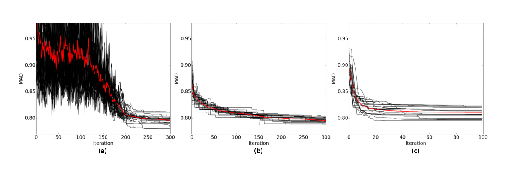
\includegraphics[width = \textwidth]{fig6.eps}
\end{figure}

Para a próxima análise assume-se a hipótese de que as escalas otimizadas e o valor ótimo de MAD, que estão inter-relacionadas, implicam em melhorias na taxa de classificação correta das espécies. Na Tabela \ref{tab:leaves_supervised_results} estão apresentados diversos valores de MAD e os correspondentes resultados em experimentos de classificação para diferentes classificadores. Observa-se que os melhores resultados de classificação correspondem aos menores valores de MAD obtidos através da otimização. Os resultados de classificação para o descritor \emph{NMBE}, com as escalas ajustadas conforme sugerido por \citeonline{Costa:1997} ($\operatorname{NMBE_{orig}}$), resultou em um desempenho intermediário quando comparado aos resultados para escalas otimizadas e escolhidas arbitrariamente. Logo, o descritor \emph{NMBE} otimizado ($\operatorname{NMBE_{opt}}$) melhorou o desempenho de todos os classificadores avaliados, uma vez que este alcançou as maiores taxas de Precisão e Revocação rates para os menores valores de MAD, o que confirma a hipótese inicial.

Apesar do descritor \emph{NMBE} ter sido originalmente projetado para descrição de neurônios, nosso trabalho aplicou-o com sucesso em caracterização de folhas de plantas, uma vez que a otimização o adequou ao problema em questão.
Embora os diferentes algoritmos de otimização tenham atingido valores de MAD diferentes, e portanto conjuntos de escalas otimizadas distintas, os resultados dos experimentos de classificação mostraram corroboraram a conclusão anterior, pois tais conjuntos de escalas foram adequadas para gerar descritores capazes de capturar informações de detalhes que diferenciem apropriadamente as formas das folhas. Logo, os algoritmos de otimização trazem vantagens à representação multiescala com impacto significativo na caracterização das folhas. 

\begin{table}[]
\begin{minipage}{\textwidth}
\renewcommand\footnoterule{}
\caption{Valores de MAD e resultados de classificação das espécies vegetais da base de imagens Flavia para diferentes estratégias de escolha das escalas do descritor \emph{NMBE}. }
\label{tab:leaves_supervised_results}
\resizebox{\textwidth}{!}{ 
\begin{tabular}{cccccccccc}
\toprule[1.5pt]
 & \multicolumn{8}{c}{Classifier} \\ \cmidrule(lr){2-9} 
 & \multicolumn{2}{c}{NB}  & \multicolumn{2}{c}{Knn (n = 5)}  & \multicolumn{2}{c}{LDA}  & \multicolumn{2}{c}{QDA} \\
\cmidrule(lr){2-3}  \cmidrule(lr){4-5} \cmidrule(lr){6-7}  \cmidrule(lr){8-9}
MAD & Precision & Recall & Precision & Recall & Precision & Recall & Precision & Recall \\ \midrule
$0,762$\footnote{Using SA}        & ${0,91 \pm 0,02}$   & ${0,89 \pm 0,02}$         & ${0,93 \pm 0,02}$          & ${0,92 \pm 0,02}$         & ${0,87  \pm 0,02}$          & ${0,85\pm 0,02}$         & ${0,95  \pm 0,01}$          & ${0,94  \pm 0,01}$         \\
$0,783$\footnote{Using DE}        & $0,88 \pm 0,02$          & $0,87\pm0,02$         & $0,90\pm0,02$          & $0,88\pm0,02$         & $0,85\pm0,02$          & $0,83\pm0,03$         & $0,91\pm0,02$          & $0,90\pm0,02$         \\
$0,829$\footnote{Using PSO}        & $0,86\pm0,03$          & $0,85\pm0,03$         & $0,89\pm0,03$          & $0,88\pm0,03$         & $0,84\pm0,03$         & $0,82\pm0,03$         & $0,91\pm0,02$          & $0,89\pm0,02$         \\
{$0,867$\footnote{Using scales proposed by \citeonline{Cesar:1996}}}          & $0,85\pm0,02$          & $0,84\pm0,02$         & $0,89\pm0,02$          & $0,88\pm0,02$         & $0,82\pm0,03$          & $0,81\pm0,03$         & $0,89\pm0,02$          & $0,88\pm0,02$         \\
{$0,969$\footnote{\label{note1}Random selection}}          & $0,81\pm0,03$          & $0,79\pm0,03$         & $0,87\pm0,02$          & $0,85\pm0,02$         & $0,77\pm0,03$          & $0,77\pm0,03$         & $0,87\pm0,03$          & $0,85\pm0,03$         \\
{$1,04$\footref{note1}}          & $0,69\pm0,03$          & $0,68\pm0,03$         & $0,83\pm0,03$          & $0,82\pm0,03$         & $0,74\pm0,03$          & $0,73\pm0,03$         & $0,81\pm0,03$          & $0,79\pm0,03$         \\
\bottomrule[1.5pt]
\end{tabular}}
\end{minipage}
\end{table}
  
Por último, observa-se que os classificadores que utilizaram descritores gerados a partir de escalas selecionadas arbitrariamente não tiveram desempenho satisfatório, pois alcançaram os menores valores de Precisão e Revocação e os maiores valores da função MAD. Portanto, escalas aleatórias levam a uma representação multiescala menos sensível a variações de características das folhas, consequentemente, mais erros de classificação. 


\section{\emph{Análise exploratória visual de agrupamentos}}
A análise exploratória visual dos agrupamentos  produzidos pela descrição NMBE das folhas indica que a descrição otimizada melhora a organização dos agrupamentos, o que reforça que a função objetivo MAD é adequada para guiar o processo de otimização desse descritor. A Figura \ref{fig:MatrizU_leaves_256}  ilustra a visualização da descrição das folhas através  das matrizes-U. Em cada posição da matriz, os valores numéricos da foram substituídos pela imagem das folhas correspondentes, estando as cores das folhas em correspondência com o rótulo das classes exibidas na Figura \ref {fig:bases}. Nessas matrizes-U estão representadas as $1907$ formas de folhas da base Flávia, sendo cada folha representada por sua descrição multiescala.

A Figura \ref{fig:MatrizU_leaves_256}a mostra a matriz-U obtida para as formas de folhas representadas pelo descritor NMBE otimizado e a Figura \ref{fig:MatrizU_leaves_256}b, pelo descritor NMBE não otimizado. Os gráficos representativos da medida \emph{silhouette} nas respectivas figuras demonstram que as classes das folhas caracterizadas e, portanto, agrupadas adequadamente são as que apresentam valores de \emph{silhouette} média positivos. Por outro lado, as classes de folhas que o descritor não foi capaz de caracterizar e agrupar adequadamente são as que apresentaram valores negativos de \emph{silhouette} média. Comparando ambas as figuras, observa-se que na Figura \ref{fig:MatrizU_leaves_256}a há expressiva redução dos valores negativos de \emph{silhouette} média para a caracterização das folhas com o descritor $\operatorname{NMBE_{opt}}$. 

\begin{figure}[t]
\caption{\label{fig:MatrizU_leaves_256} Matrizes-U e a \emph{silhouette} média para as descrições das folhas da base Flavia com o descritor NMBE (a) optimizado e (b) não otimizado.}
\centering
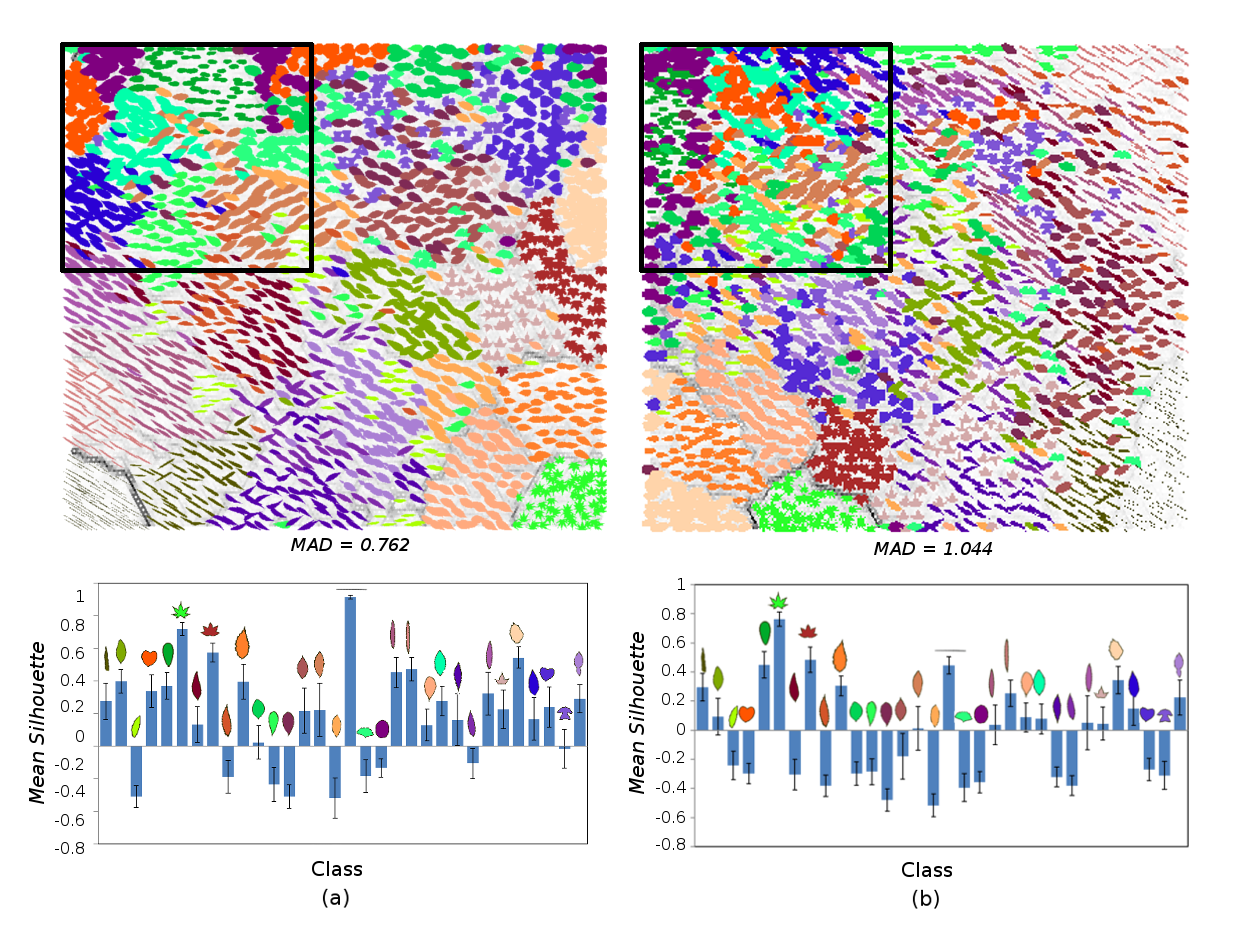
\includegraphics[width=\textwidth]{fig7.eps}
\end{figure}
}
{\color{red}
The black square in Figure \ref{fig:MatrizU_leaves_256}a highlights  the performance of the optimized descriptor. It also shows how well the optimized descriptor mapped leaf shapes into groups according to their respective classes.  Moreover, the optimized descriptor has remarkably improved  the mean \emph{silhouette} per class for almost all leaf classes. In contrast, the region inside the black square in Figure \ref{fig:MatrizU_leaves_256}b indicates that the non-optimized descriptor was unable to satisfactorily map leaf shapes in their corresponding classes.
These results  indicated that the optimized descriptor has improved the cluster arrangement of leaves due to the intrinsic shape variations within the set of optimized scales that can not be properly embodied in the studied traditional parameter selection methods.

Figures \ref{fig:MatrizU_leaves_II}a, \ref{fig:MatrizU_leaves_II}b and \ref{fig:MatrizU_leaves_II}c display the U-matrices and the corresponding MAD values for experiments on Flavia leaf data set with SA, DE and PSO, respectively. An interesting aspect to examine in these results regards the convergence of the optimization algorithms to different solutions (MAD). These solutions resulted in different cluster arrangements and therefore different relations among the neighborhood structure of clusters. For instance, the overall dispersion  of the elements in Figure \ref{fig:MatrizU_leaves_II}a and Figure \ref{fig:MatrizU_leaves_II}b tend to be very similar since  the corresponding MAD values are close to each other. At the same time, the result that corresponds to the highest MAD value ($0.829$) exhibits a relatively high dispersion within clusters, particularly at the center of the U-matrix (Figure \ref{fig:MatrizU_leaves_II}c), which reinforces the hypothesis that  PSO converged to a local minimum. These findings point to the important conclusion that the lower the MAD value, the better the cluster arrangement and hence the cluster quality. Therefore, we state that the cluster quality and MAD value are negatively correlated. Our analysis also considers that there are other solutions than the minimum, in the search space, which may be suitable to the problem under study. 

\begin{figure}[h!]
 \caption{\label{fig:MatrizU_leaves_II}Matrices-U e valores MAD obtidos para a base de imagens Flavia por uso da NMBE otimizada pelos algoritmos (a) SA, (b) DE, (c) PSO.}
\centering
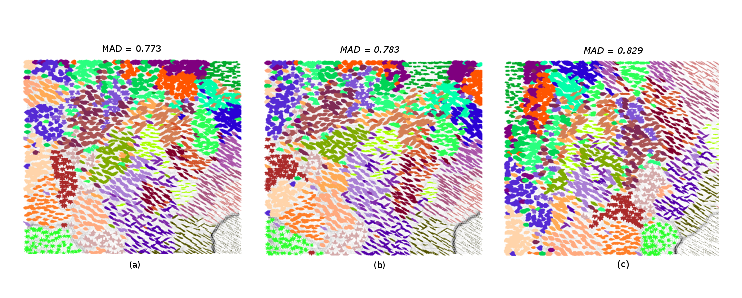
\includegraphics[width=\textwidth,trim = 0mm 0mm 0mm 4.5mm,clip]{fig8.eps}
\end{figure}

Figure \ref{MDS:Leaves} illustrates the MDS projections for three different MAD values. Figure \ref{MDS:Leaves}a corresponds to the cluster arrangement after the convergence of the SA algorithm, i.e. after reaching the minimum MAD value. These projections confirmed that the minimization of the objective function provided leaf cluster arrangements with lower average within-class distances and higher inter-class distances, and thus  more compact and separated clusters. The visual analysis of the three detail images in Figure \ref{MDS:Leaves}a discloses that the MDS projection of the optimized NMBE descriptor increased inter-class distances, whereas it reduced the within-class distances when compared to Figure \ref{MDS:Leaves}b and \ref{MDS:Leaves}c. Moreover, the $R^2$ coefficient values close to 1 imply that the low-dimensional representation preserved the mean distance in the original high-dimensional data space.

\begin{figure}[h!]
 \caption{\label{MDS:Leaves} Projeções MDS dos descritores NMBE para formas da base de folhas Flavia. (a) Descritor NMBE otimizado pelo algoritmo SA com valor de função $MAD = 0,762$ (b) Descritor NMBE não otimizado com valor de função $MAD =0,969$ and (c) Descritor NMBE não otimizado com valor de função $MAD = 1,044$.}

\centering
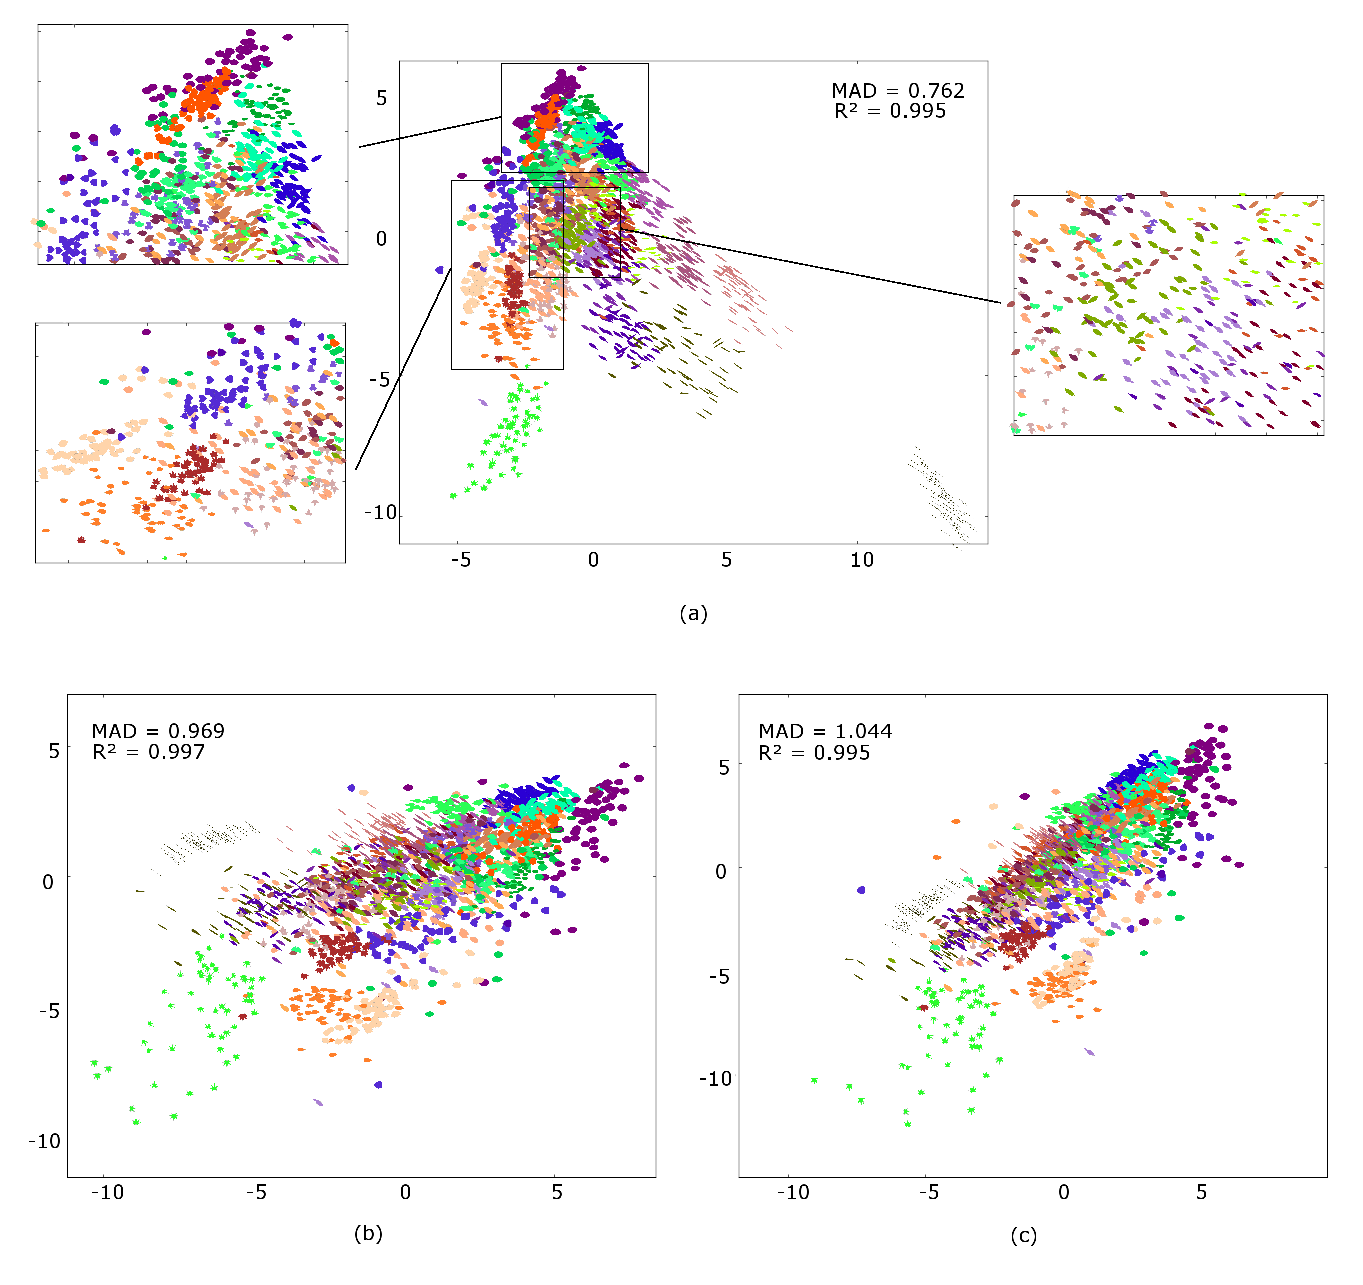
\includegraphics[width=\textwidth]{fig9.eps}
\end{figure}
\section{\emph{Recuperação de imagens baseada em conteúdo - CBIR}}
For the sake of comparison, we have optimized the parameters of another shape descriptor namely inner distance shape context (IDSC) \citeonline{Ling:2007:SCU:1191552.1191806}.
This descriptor is mainly applied to shape retrieval, which involves unsupervised shape classification tasks.  Moreover, IDSC employs dynamic programming (DP), such as Dynamic Time Warping (DTW) \citeonline{PalazonGonzalez2012978}, to improve shape matching accuracy. In this paper, we have replaced the $L_2$ norm by DTW to compute the \emph{silhouette} measure and the cost function defined in equation \ref{eq:mad}.  
Figure \ref{figfig1Optmization-IDSC} exhibits the comparison of shape retrieval experiments which were performed on the public Flavia leaf data set and with both non-optimized NMBE and IDSC and their optimized counterparts ($\operatorname{NMBE_{opt}}$, $\operatorname{IDSC_{opt}}$).
The performance evaluation methodology has adapted the Bulls-eye measure, where the result is the overall number of shapes correctly  retrieved, in each rank position, for each shape in data set taken as a query.  Let $N_c$ be the number of shapes which belong to the class $c$. Here, the number of retrieved shapes ($N_r$) was adjusted to $N_r = 2\displaystyle \min_{c = 1,2,\dots 32}{N_c}$. Figure \ref{figfig1Optmization-IDSC} also demonstrates that the optimization methodology was decisive for both descriptors to achieve better retrieval rates. 
Figure \ref{fig1Ooptimization_graph}  shows that after tuning IDSC parameters for the Flavia leaf data set with the optimization methodology the retrieval rate has remarkably increased. Therefore, $\operatorname{IDSC_{opt}}$  outperformed the optimized NMBE ($\operatorname{NMBE_{opt}}$) and non-optimized NMBE. In this sense, the optimized parameters of $\operatorname{IDSC_{opt}}$ may have incorporated subtle details of leaf shapes. On the other hand, we have observed that the non-optimized IDSC underperformed the non-optimized NMBE. 
In order to provide a non-optimized counterpart of IDSC, we have followed the parameter setting introduced in \citeonline{wang2015march}.
Figure \ref{subfig:upper-right} and \ref{subfig:lower-right} exemplify samples of  plant leaves which were retrieved according to the rank of the similarity to the two queries. These results have demonstrated that the non-optimized descriptors in Figure \ref{subfig:upper-right} and \ref{subfig:lower-right} were unable to retrieve all samples for the two queries, whereas the  optimized descriptors retrieved all of them, correctly.

\begin{figure}[]
\caption{Experimentos realizados com formas da base de imagens de folhas Flavia (a) taxa de recuperação  obtida com os descritores NMBE e IDSC originais e suas versões otimizadas, (b) e (c)recuperação de duas amostras de folhas utilizando os descritores NMBE e IDSC otimizados e não otimizados, respectivamente.  respectively.\label{fig1Ooptimization_graph}}
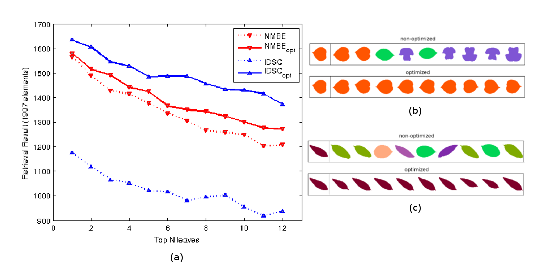
\includegraphics[width=\textwidth]{fig10.eps}
\end{figure}

\begin{comment}
\begin{figure}[t!]
\begin{subfigure}{0.55\textwidth}
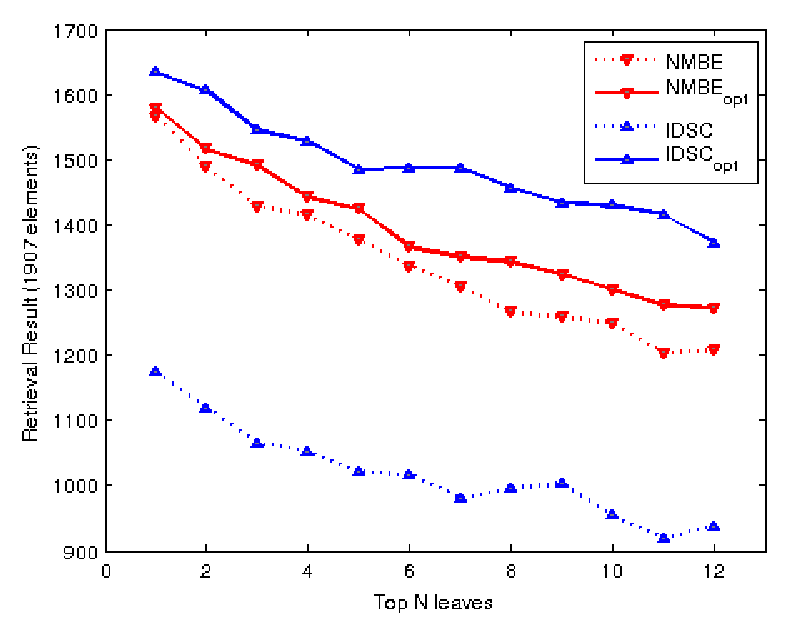
\includegraphics[width=\textwidth]{fig10a.eps}
\caption{Retrieval rates. \label{fig1Ooptimization_graph}}
\end{subfigure}
\hspace*{\fill}
\begin{minipage}{0.45\textwidth}
\begin{subfigure}{\textwidth}
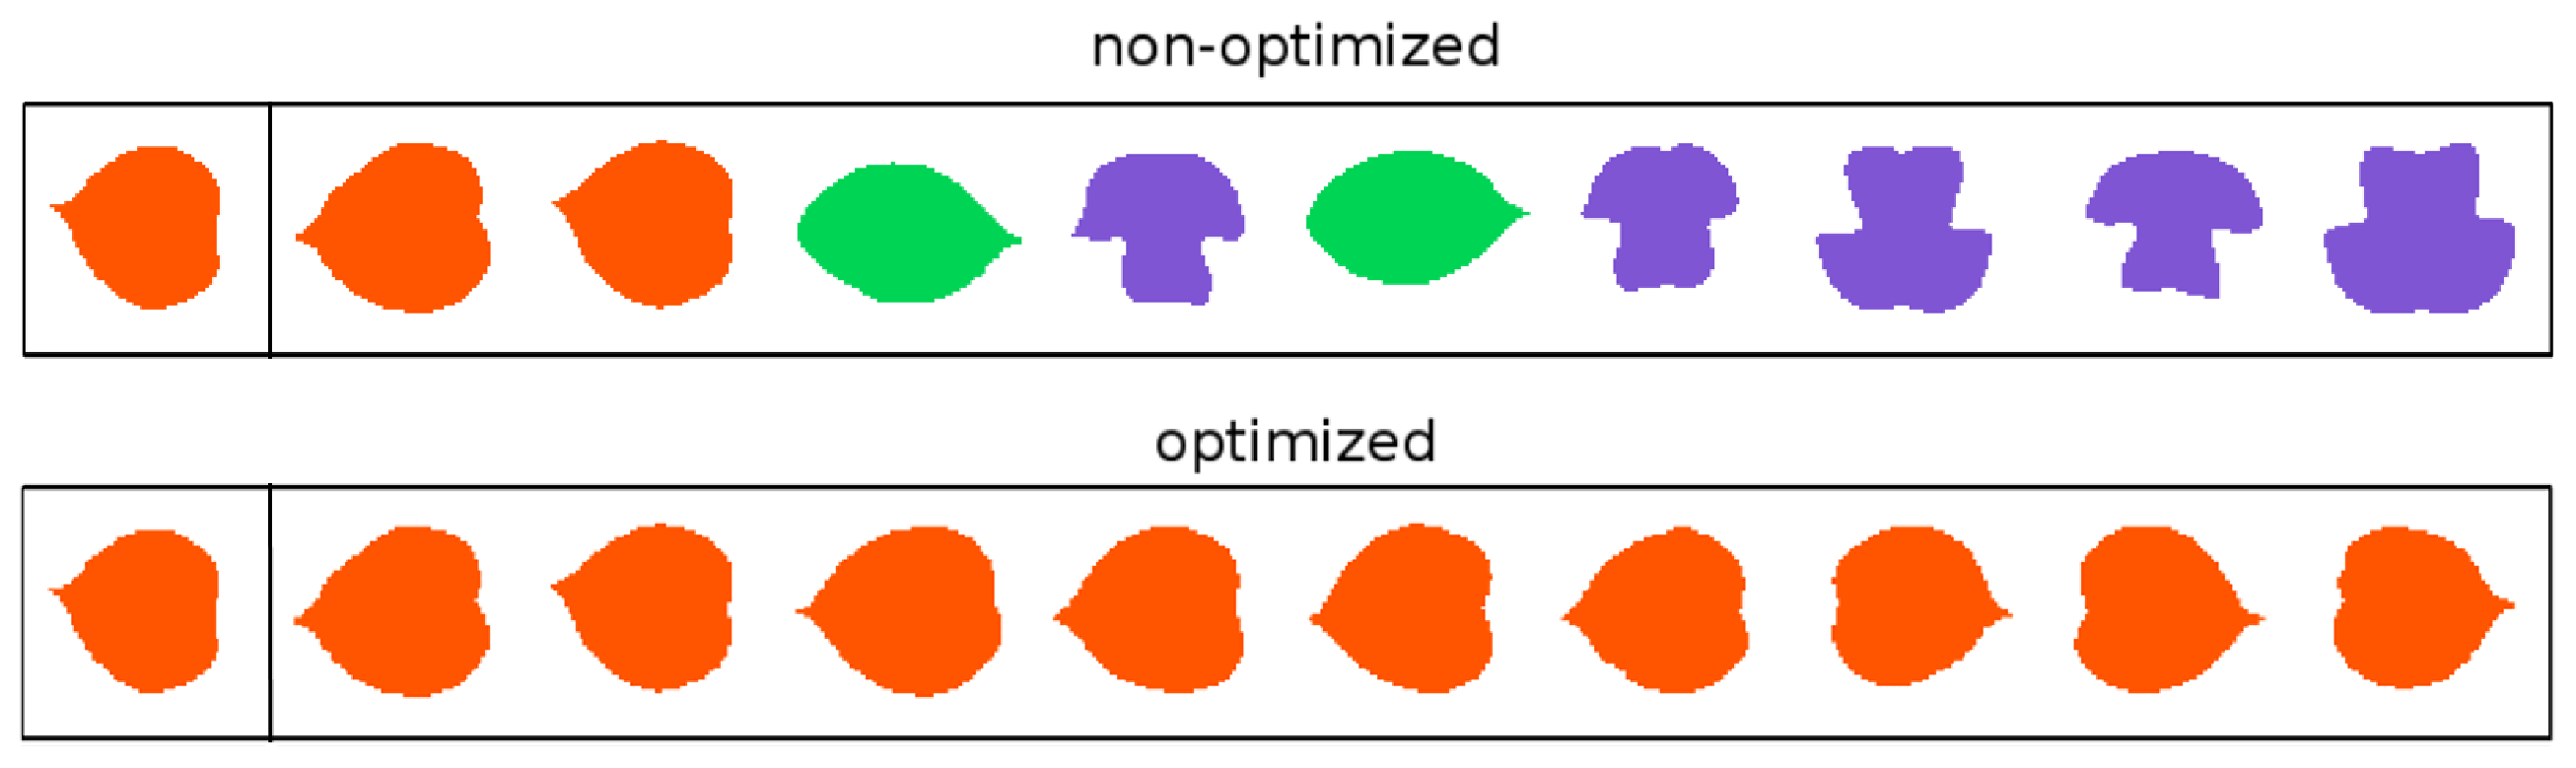
\includegraphics[width=\textwidth]{fig10b.eps}
\caption{Retrieval results with NMBE.} \label{subfig:upper-right}

\end{subfigure}

\vspace*{0.60cm}
\begin{subfigure}{\textwidth}
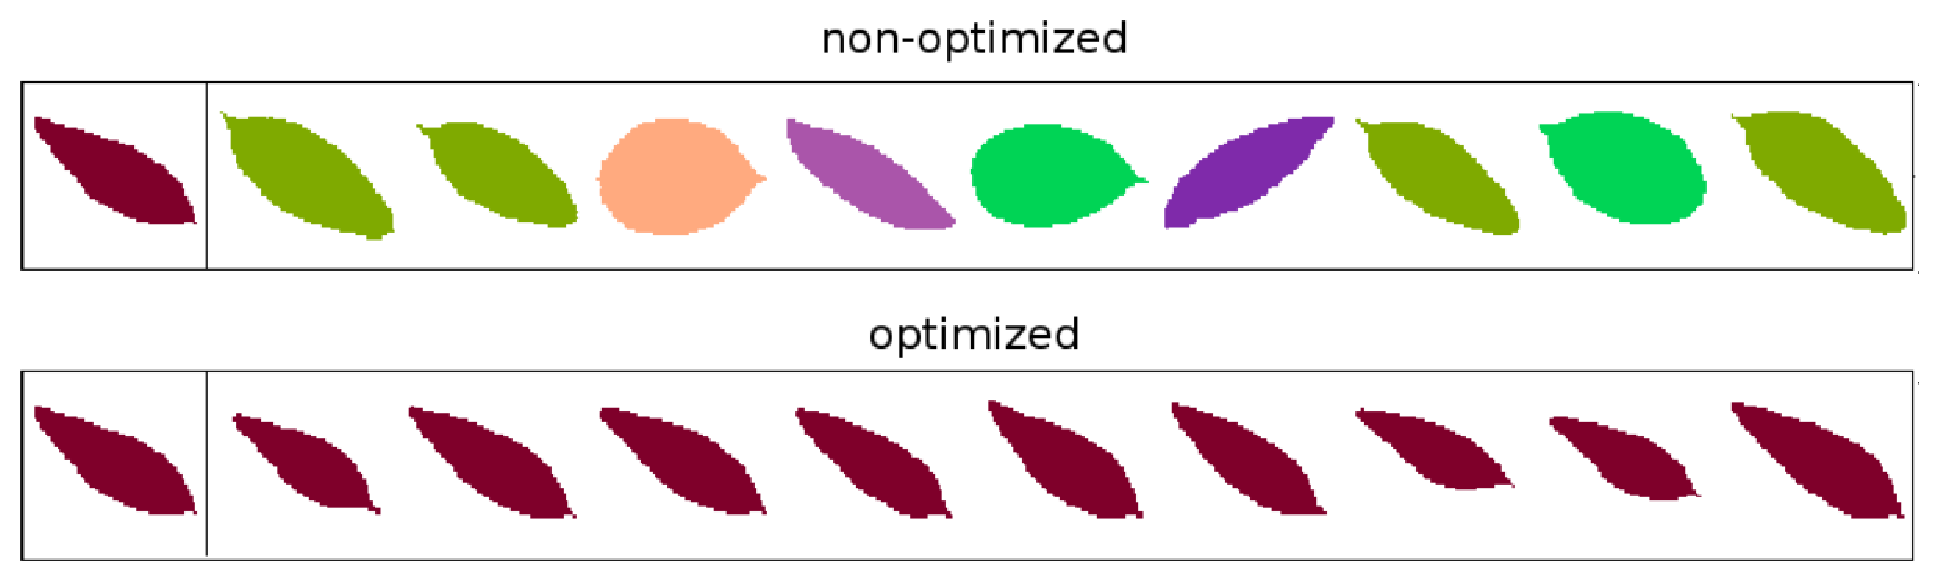
\includegraphics[width=\textwidth]{fig10c.eps}
\caption{Retrieval results with IDSC.\label{subfig:lower-right}}
\end{subfigure}
\end{minipage}

\caption{\label{figfig1Optmization-IDSC} Experiments conducted on Flavia leaf data set (a) retrieval rate by using both NMBE and IDSC and their optimized counterparts, (b) and (c) two leaf shape retrieval examples by using the non-optimized and optimized NMBE and IDSC descriptors, respectively.} 
\end{figure}
\end{comment}

 Table \ref{table_bull_eyes_leaves} presents the performance evaluation of NMBE, whose scales were computed using the scheme introduced by \citeonline{Cesar:1996}, IDSC and their optimized counterparts.  The retrieval rates show that both optimized descriptors outperformed their non-optimized counterparts on Flavia data set. The remarkable improvement on the Bulls-eye rates reinforces our assumption that the optimization methodology is suitable for leaf shape retrieval and analysis.

\begin{table}[h!]
\centering
\caption{Taxa Bulls-eye para a base de imagens Flavia.}
\label{table_bull_eyes_leaves}
  \begin{tabular}{cccccccc}
  \toprule[1.5pt]
 $\operatorname{NMBE}$ & $\operatorname{NMBE_{opt}}$ & IDSC    & $\operatorname{IDSC_{opt}}$\\ \midrule
     63.86 \%  & 71.16 \%  & 53.38\%    & 77.50\%       \\
  \bottomrule[1.5pt]
  \end{tabular}
\end{table}

Thus, we can infer that the optimized descriptors are more likely to succeed in shape retrieval experiments because the optimized sets of parameters probably embody intrinsic and subtle information about leaf shapes. We can also assume that these optimized descriptors may reliably characterize and also discriminate shape differences within and among leaf classes. 

\subsection{Computational cost \label{sec:comp_cost}}

Table \ref{tbl:complexity} shows the computational complexity results of the three optimization algorithms. SA and PSO present similar complexity results which rely on the number of iterations to converge ($N_{iter}$), population size ($N_{pop}$) and $P$ parameter. On the other hand,  DE  demands a higher complexity which relies on the dimension of the optimization problem ($D$), population size ($N_{pop}$) and number of iterations to converge ($N_{iter}$).

\begin{table}[h!]
\centering
\caption{Complexidade computacional dos métodos de otimização.}
\label{tbl:complexity}
  \begin{tabular}{ll}
  \toprule[1.5pt]
 Método & Complexidade\\
 \midrule
   SA  & $O(P.N_{iter}.\log{N_{iter}})$    \\
   DE  & $O(N_{pop}.N_{iter}.D)$   \\
   PSO&  $O(N_{pop}.N_{iter}.\log{N_{iter}})$\\
  \bottomrule[1.5pt]
  \end{tabular}
\end{table}

For the sake of comparison, we assumed that the computational cost is the number of times that the objective function is demanded throughout the optimization process. Its calculation takes into account the parameter setting of each method, presented in Section \ref{subsec:opmet}, and the corresponding computational complexity.  The computational cost to address the optimization of the multiscale descriptor for SA, DE and PSO yielded $7,4314$, $19,500$ and $1,107$, respectively. 

It is worth noting that there is a trade-off between the computational cost and the quality of the optimal solution found. Although the reduction of the number of shape samples, image resolution and the $N_{pop}$ variable can lessen the computational cost, it may degrade the optimization result. Moreover, parallelism may contribute to reduce the computational cost without degrading the optimization result.  However, it adds an extra computational complexity to the optimization algorithms.
}


%\section{Visualização dos dados}

%\subsection{\emph{DFM}}


Com base na metodologia exposta apresentamos neste capítulo os resultados experimentais obtidos na análise dos descritores dimensão fractal multiescala, energia de dobramento multiescala Uma avaliação comparativa dos resultados obtidos com os descritores \emph{NMBE} e \emph{DFM} é apresentada na seção a seguir.

\begin{figure}
 \caption{\label{fig:dfm99} (a) Matriz-U para as formas da base Kimia99 representadas com o descritor dimensão fractal multiescala. (b) \textit{Silhouette} média por classe obtida a partir do referido descritor.}
  \centering
  \includegraphics[width=\textwidth]{dfm99.png}
\end{figure}

\begin{figure}
 \caption{\label{fig:dfm216} (a) Matriz-U para as formas da base Kimia216 representadas com o descritor dimensão fractal multiescala. (b) \textit{Silhouette} média por classe obtida a partir do referido descritor.}
  \centering
  \includegraphics[width=\textwidth]{dfm216.png}
\end{figure}

\begin{figure}
 \caption{\label{fig:nmbe99} (a) Matriz-U para as formas da base Kimia99 representadas com o descritor energia de dobramento multiescala. (b) \textit{Silhouette }média por classe obtida a partir do referido descritor.}
  \centering
  \includegraphics[width=\textwidth]{nmbe99.png}
\end{figure}

\begin{figure}
 \caption{\label{fig:nmbe216} (a) Matriz-U para as formas da base Kimia216 representadas com o descritor energia de dobramento multiescala. (b) Silhouette média por classe aferida a partir do descritor}
  \centering
  \includegraphics[width=\textwidth]{nmbe216.png}
\end{figure}


\begin{comment}
\begin{figure}
 \caption{\label{fig:edif99} (a) Matriz-U para as formas da base Kimia99 representadas com o descritor entropia multiescala. (b) Silhouette média por classe aferida a partir do descritor}
  \centering
  \includegraphics[width=\textwidth]{ediferencial99.png}
\end{figure}

\begin{figure}
 \caption{\label{fig:edif216} (a) Matriz-U para as formas da base Kimia216 representadas com o descritor entropia multiescala. (b) Silhouette média por classe aferida a partir do descritor}
  \centering
  \includegraphics[width=\textwidth]{ediferencial216.png}
\end{figure}

\begin{figure}
 \caption{\label{fig:edis99} (a) Matriz-U para as formas da base Kimia99 representadas com o descritor entropia multiescala. (b) Silhouette média por classe aferida a partir do descritor}
  \centering
  \includegraphics[width=\textwidth]{ediscreta99.png}
\end{figure}

\begin{figure}
 \caption{\label{fig:edis216} (a) Matriz-U para as formas da base Kimia216 representadas com o descritor entropia multiescala. (b) Silhouette média por classe aferida a partir do descritor}
  \centering
  \includegraphics[width=\textwidth]{ediscreta216.png}
\end{figure}

\subsection{\emph{NMBE} e \emph{DFM}}
Os experimentos de avaliação de desempenho dos descritores produziram como saída as matrizes-U que estão apresentadas na Figuras \ref{fig:nmbe_som_map}, \ref{fig:mfd_som_map} e  \ref{fig:som_kimia_216}. Nas Figuras \ref{fig:nmbe_som_map} e \ref{fig:mfd_som_map}, as regiões delimitadas com linhas tracejadas correspondem as classes de formas com os maiores valores médios da medida Silhouette (Figuras \ref{fig:silhouette}a e \ref{fig:silhouette}b). Nesses casos pode-se deduzir que ambos os descritores foram capazes de caracterizar corretamente estas classes de formas.

Já os grupos delimitados com linhas contínuas referem-se às classes de formas com os menores valores de Silhouette média. De fato, as formas dessas classes aparecem nas matrizes-U dispersas em sub-grupos, que é um indicativo que ambos os descritores falharam em caracterizá-las adequadamente.
  
As Figuras \ref{fig:dude_tool_mfd} e \ref{fig:dude_tool_nmbe} mostram objetos das classes de formas de humanos e ferramentas. Ambos os descritores foram capazes de discriminar os objetos das referidas classes, como evidenciado nos gráficos apresentados. As matrizes-U (Figuras \ref{fig:nmbe_som_map} e \ref{fig:mfd_som_map}) também confirmam esse resultado exibindo, para essas classes de formas, homogeneidade intra-classe e separabilidade inter-classes. Logo, concluímos que estes descritores são efetivos em representar formas para o reconhecimento de padrões em aplicações \emph{CBIR}.

Também evidenciamos nas Figuras \ref{fig:mfd_som_map} e \ref{fig:nmbe_som_map} que o descritor \emph{DFM} apresentou maior dispersão inter-classe para as formas de humanos que o descritor \emph{NMBE}. Essa observação é consistente com os resultados obtidos através da medida \emph{Silhouete}, aonde o valor dessa medida para formas humanas descritas com a \emph{DFM} é menor do que o valor para essas mesmas formas descritas com a \emph{NMBE}.

Ademais, os sinais em linhas tracejadas vermelhas e em linhas contínuas azuis, apresentados nas Figuras \ref{fig:dude_tool_mfd} e \ref{fig:dude_tool_nmbe}, mostram que o descritor \emph{NMBE} é mais robusto a diferenças intra-classe que o descritor \emph{DFM}. Nesses gráficos, as formas pertencentes a mesma classe que o descritor representa seguindo um mesmo padrão apresentam-se próximas umas das outras na matriz-U, enquanto as formas que o descritor representa divergindo do padrão são mapeadas na matriz-U distantes dos grupo correspondente. Exemplos desta última condição são as formas humanas rotuladas como $2$ e $4$ nas Figuras \ref{fig:dude_tool_mfd} e \ref{fig:dude_tool_nmbe}.


Furthermore, there is a larger variation among tools descriptions in the graphs of  the figure \ref{fig:descritores}a than the  variations observed in the graphs of the figure \ref{fig:descritores}b. Coherently, the corresponding shapes appears in the U-matrix more dispersed  for the \emph{MFD} description than for the \emph{NMBE} description.

\begin{figure}[h!]
  \caption{\label{fig:nmbe_som_map} Matriz-U para as formas da base Kimia99 representadas com o descritor Energia de dobramento multiescala.}
  \centering
  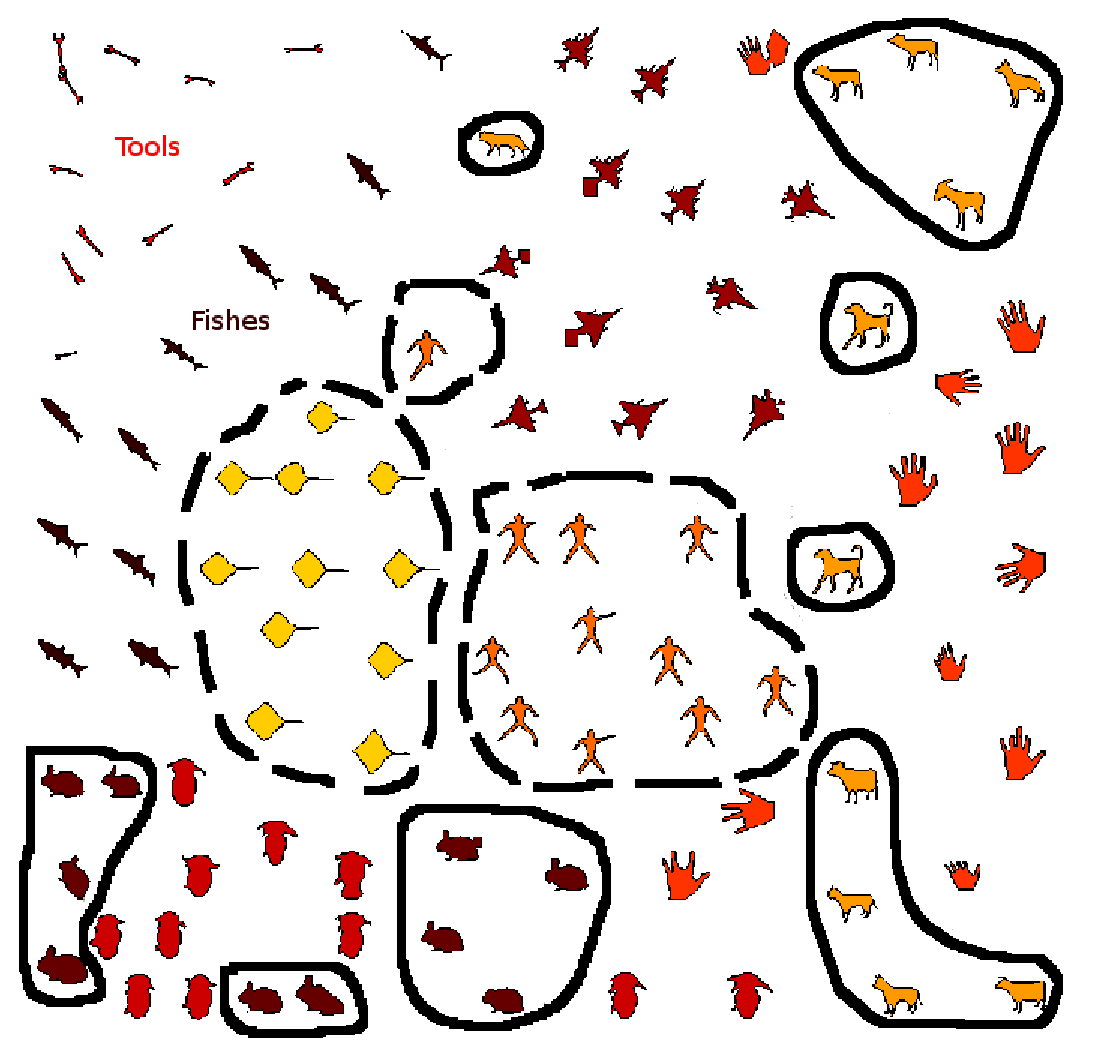
\includegraphics[width=0.5\textwidth]{nmbe_som_map_v4.eps}
\end{figure}

\begin{figure}[h!]
  \caption{\label{fig:mfd_som_map} Matriz-U para as formas da base Kimia99 representadas com o descritor Dimensão fractal multiescala.}
  \centering
  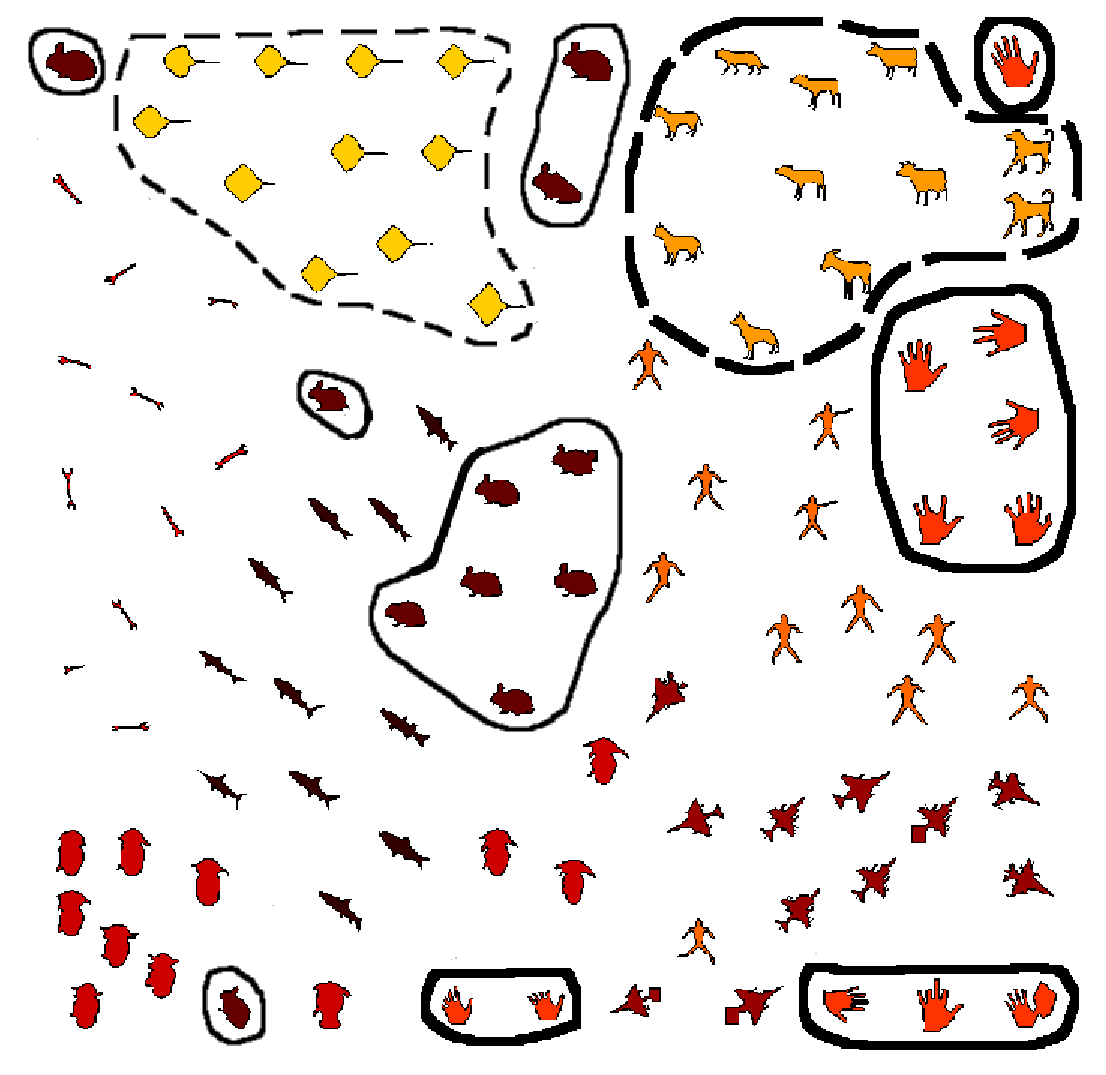
\includegraphics[width=0.5\textwidth]{mfd_som_map_v3.eps}
\end{figure}
  
\begin{figure}[h!]  \caption{\label{fig:som_kimia_216} Para o descritor energia de dobramento multiescala e a base Kimia-216: (a) Matriz-U. (b) Alguns resultados de recuperação de formas pelo conteúdo.}
  \centering
  \includegraphics[width=0.5\textwidth]{retr_som_kimia216_v2.png}
\end{figure}

Já a Figura \ref{fig:som_kimia_216}a apresenta os resultados da visualização das formas da base Kimia-216 representadas através do descritor \emph{NMBE}. No canto inferior direito desta figura observamos que o descritor confunde formas dos elefantes com as dos camelos. Essa confusão aparece também no experimento de recuperação de formas pelo conteúdo (Figura \ref{fig:som_kimia_216}b), em que uma dentre as formas dos elefantes é utilizada como protótipo para se recuperar as onze formas mais similares ao protótipo na referida base.

Analogamente, no canto superior esquerdo da Figura \ref{fig:som_kimia_216}a, há confusão entre os agrupamentos das formas das faces e dos corações, bem como a presença duma forma de garfo. Na segunda linha da Figura \ref{fig:som_kimia_216}b observamos a presença dessas formas indesejáveis no experimento de recuperação de formas quando uma forma de face é apresentada como protótipo. 

Os demais resultados de recuperação de formas, apresentados na Figura \ref{fig:som_kimia_216}b, também estão coerentes com as observações da matriz-U. Nessa última podemos observar que o grupo das formas das arraias são mapeadas vizinhas aos grupos das formas dos cálices e dos pássaros, o que resulta no aparecimento das formas dessas últimas classes quando se realiza a recuperação de arraias. 

Outro aspecto importante de ser observado é que  grupos de formas com similaridades grosseiras encontram-se mapeados próximos uns dos outros na matriz-U. Formas alongadas, por exemplo, estão organizadas na parte inferior esquerda da Figura \ref{fig:som_kimia_216}a, enquanto formas arredondadas encontram-se na parte superior. Outros exemplos incluem os seguintes grupos: chaves e crianças (esquerda da figura), carros e tijolos, tartarugas e pássaros, cálices e sepulturas. 

\begin{figure}[h!]
  \caption{\label{fig:silhouette} Silhouette média por classe aferida, com a base Kimia-99, para os descritores (a) Dimensão fractal multiescala; (b) Energia de dobramento multiescala.}
  \centering
  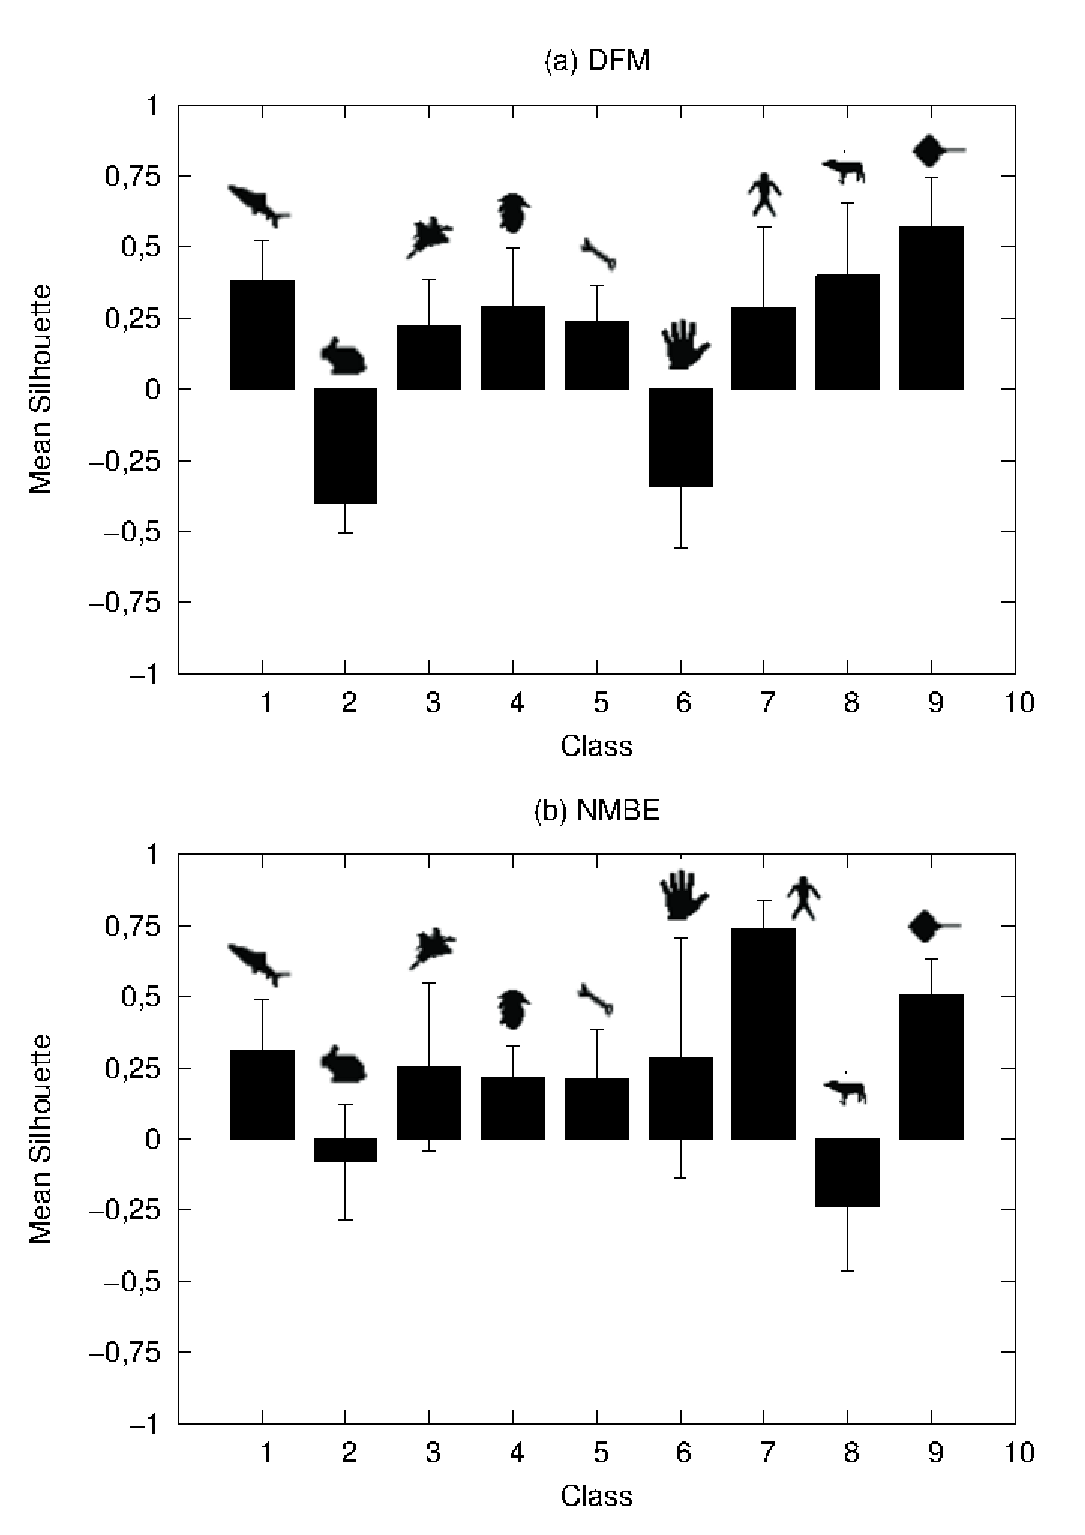
\includegraphics[width=0.5\textwidth]{resultado_silhouette.eps}
\end{figure}

\begin{figure}[h!]
  \caption{\label{fig:dude_tool_mfd}   Vetores de características calculados para amostras das formas de humanos e de ferramentas com o descritor dimensão fractal multiescala.}
  \centering
  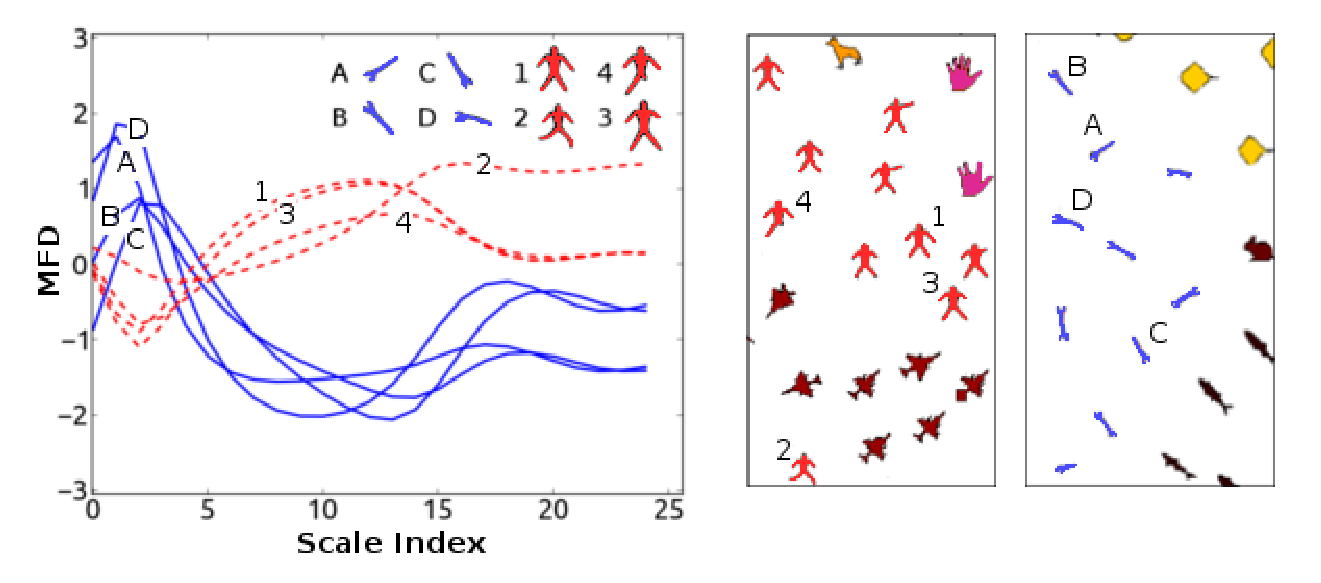
\includegraphics[width=0.75\textwidth]{dude_tool_mfd_v6.eps}
\end{figure}

\begin{figure}[h!]
  \caption{\label{fig:dude_tool_nmbe} Vetores de características calculados para amostras das formas de humanos e de ferramentes com o descritor energia de dobramento multiescala.}
  \centering
  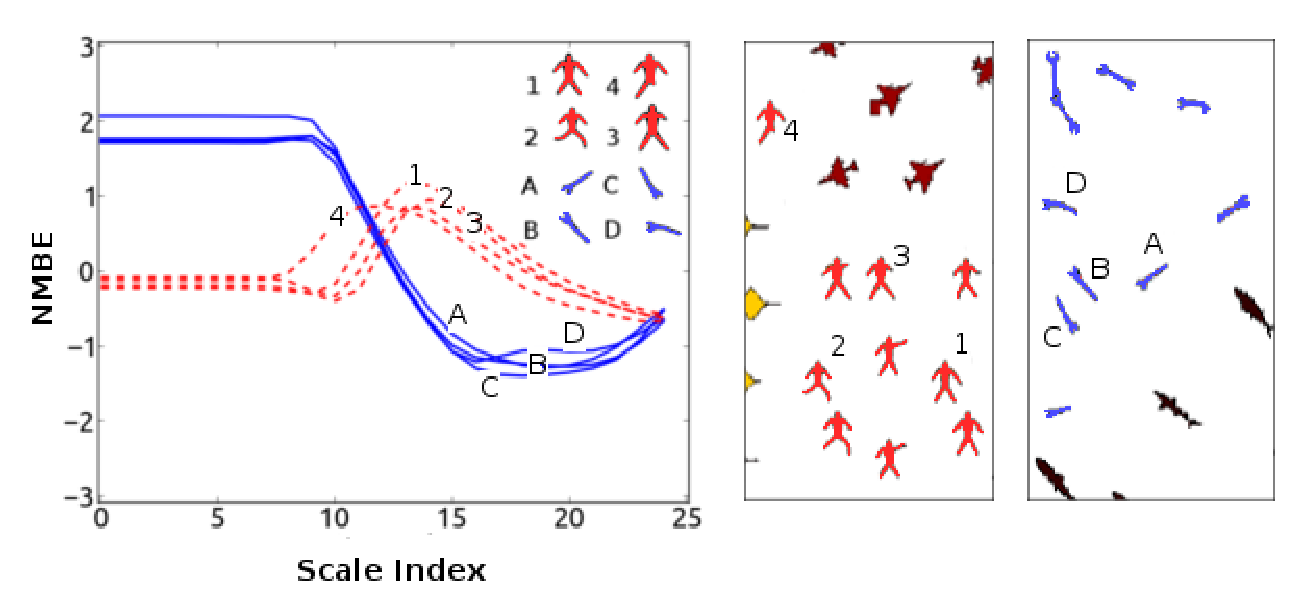
\includegraphics[width=0.75\textwidth]{dude_tool_nmbe_v6.eps}
\end{figure}

\subsection{Entropia diferencial da curvatura multiescala}

A visualização de dados obtida para características extraídas com o descritor entropia diferencial da curvatura multiescala, para a base Kimia-99, está apresentada na Figura \ref{fig:edif99}a. Nesta figura observamos a Matriz-U, em tons de cinza, sobreposta às figuras das formas nas posições mapeadas pela rede SOM.

As células escuras formam contornos que delimitam fronteiras existentes entre agrupamentos de formas, pois estas células indicam a existência duma relação de separação entre as formas em suas vizinhanças. Já as células em linhas claras indicam maior proximidade entre as formas e suas vizinhanças.

Podemos inferir que o descritor representou adequadamente as formas das classes de humanos, arraias, peixes, ferramentas e coelhos. Isso porque, nestes casos, o descritor apresentou uma representação compacta, agrupando próximas as formas de uma mesma classe, e propiciando separabilidade entre os agrupamentos estabelecidos. A medida Silhouette média por classe, apresentada na Figura \ref{fig:edif99}b, corrobora nossas observações, pois as referidas classes são as que apresentam os valores de Silhouette média mais positivos e com pequeno desvio padrão.  

Por outro lado, o descritor falhou em representar as formas das classes de animais quadrúpedes, aviões e extra terrestres. Isso porque, nesses casos, não se consegue identificar na matriz-U fronteiras claras que estabeleçam um único agrupamento das formas de uma mesma classe. Em outras palavras, formas dessas classes encontram-se separadas umas das outras ou dispersas em sub-grupos delimitados por pequenas fronteiras. Esses casos são os que apresentam a medida Silhouette média por classe com os menores valores e os maiores desvios padrão. 

Já na Figura \ref{fig:edif216}a temos a visualização da matriz-U para as características extraídas das formas da base Kimia-216. Nesta observamos, bem delimitados por linhas escuras, diversos agrupamentos  representados corretamente pelo descritor. Dentre esses, destacamos os agrupamentos cujas fronteiras de separação intra-classe são de baixo contraste e cujas fronteiras de separação inter-classe são bem contrastadas (faces, garfos, sepulturas, cálices e crianças). Esses são os  agrupamentos que apresentaram os maiores valores de \emph{Silhouette} média na Figura \ref{fig:edif216}b, o que é um resultado esperado, uma vez que o descritor representou as formas desses grupos de forma compacta e em agrupamentos bem separados.

\begin{figure}
\caption{\label{fig:edif_som_map} Matriz-U para as formas da base Kimia99 representadas com o descritor Entropia diferencial da curvatura multiescala.}
  \centering
  \includegraphics[width=\textwidth]{ediferencial_N5_formas.png}
 \end{figure}

\begin{figure}
\caption{\label{fig:silhouette_ediferencial} Silhouette média por classe aferida, com a base Kimia-99, para o descritor entropia diferencial da curvatura multiescala.}
  \centering
  \includegraphics[width=0.75\textwidth]{ediferencial_silhouette_N5.png}
\end{figure}

\begin{figure}[h!]
  \caption{\label{fig:som_nmbe} Visualização dos dados obtida com o mapa auto-organizável de Kohonen para a descrição \emph{NMBE}.}
  \centering
  \includegraphics[width=0.5\textwidth]{mapa_som_descritor_nmbe.png}
\end{figure}

\begin{figure}[h!]
  \caption{\label{fig:som_dfm} Visualização dos dados obtida com o mapa auto-organizável de Kohonen para a descrição \emph{NMBE}.}
  \centering
  \includegraphics[width=0.5\textwidth]{mapa_som_descritor_dfm.png}
\end{figure}

\section{Recuperação de imagens pelo conteúdo}

\begin{table*}
\centering
\caption{\label{tab:KimiaChernoff} Total de acertos por classe e por posição, nos experimentos \emph{CBIR}, com a distância de Chernoff.}
\begin{tabular}{l| r r r r r r r r r r r}
\hline
&\multicolumn{11}{l}{nth nearest match} \\
\cline{2-12}
Classe&1&2&3&4&5&6&7&8&9&10&11 \\
 \hline
Peixes&11&11&11&11&9&5&8&3&7&5&5\\
Coelhos&11&11&11&11&11&11&11&11&11&11&7\\ 
Aviões&11&10&8&8&7&7&7&5&2&1&1\\
ETs&11&11&11&11&11&11&11&11&8&7&5\\
Ferramentas&11&8&7&10&3&9&9&5&7&9&9\\
Mãos&11&11&11&11&11&11&11&11&11&9&7\\
humanos&11&11&11&11&11&11&11&11&11&11&11\\
Quadrupedes&11&11&9&8&8&7&8&3&5&8&4\\
Arraias&11&11&11&11&11&11&11&10&11&9&7\\
\hline
Total&99&95&90&92&82&83&87&70&73&70&56\\
\hline
\end{tabular}
\end{table*}

\begin{table*}
\centering
\caption{\label{tab:KimiaChi-square} Total de acertos por classe e por posição, nos experimentos \emph{CBIR}, com a distância de Chi-square.}
\begin{tabular}{l| r r r r r r r r r r r}
\hline
&\multicolumn{11}{l}{nth nearest match} \\
\cline{2-12}
Classe&1&2&3&4&5&6&7&8&9&10&11 \\
 \hline
Peixes&11&11&11&10&10&8&7&9&4&4&3\\
Coelhos&11&10&10&10&10&10&10&10&10&8&1\\ 
Aviões&11&11&11&9&9&9&8&5&2&2&2\\
ETs&11&11&11&10&11&10&11&10&10&8&7\\
Ferramentas&11&11&11&11&11&11&11&11&10&11& 11\\
Mãos&11&11&11&11&11&11&11&11&11&11&9\\
humanos&11&11&11&11&11&11&11&11&11&11&11\\
Quadrupedes&11&11&6&9&8&7&7&5&7&7&4\\
Arraias&11&11&11&11&11&11&11&10&11&11&10\\
\hline
Total&99&98&93&92&92&88&87&82&76&73&58\\
\hline
\end{tabular}
\end{table*}

\begin{table*}
\centering
\caption{\label{tab:KimiaHellinger} Total de acertos por classe e por posição, nos experimentos \emph{CBIR}, com a distância de Hellinger.}
\begin{tabular}{l| r r r r r r r r r r r}
\hline
&\multicolumn{11}{l}{nth nearest match} \\
\cline{2-12}
Classe&1&2&3&4&5&6&7&8&9&10&11 \\
 \hline
Peixes&11&11&11&10&10&9&5&8&8&2&2\\
Coelhos&11&11&11&11&11&10&10&10&11&8&2\\ 
Aviões&11&11&11&10&9&11&9&8&1&1&0\\
ETs&11&11&11&11&10&11&10&11&11&7&4\\
Ferramentas&11&11&11&11&11&11&11&10&11&11& 10\\
Mãos&11&11&11&11&11&11&11&11&11&11&8\\
humanos&11&11&11&11&11&11&11&11&11&11&11\\
Quadrupedes&11&11&7&9&6&6&5&7&9&5&4\\
Arraias&11&11&11&11&11&11&11&11&11&10&9\\
\hline
Total&99&99&95&95&90&91&83&87&84&66&50\\
\hline
\end{tabular}
\end{table*}

\begin{table*}
\centering
\caption{\label{tab:KimiaJensen-Shannon} Total de acertos por classe e por posição, nos experimentos \emph{CBIR}, com a distância Jensen-Shannon.}
\begin{tabular}{l| r r r r r r r r r r r}
\hline
&\multicolumn{11}{l}{nth nearest match} \\
\cline{2-12}
Classe&1&2&3&4&5&6&7&8&9&10&11 \\
 \hline
Peixes&11&11&11&10&10&8&7&7&7&4&1\\
Coelhos&11&10&10&10&10&10&10&10&9&8&2\\ 
Aviões&11&11&10&10&9&8&8&6&3&1&1\\
ETs&11&11&11&10&11&10&10&11&9&8&5\\
Ferramentas&11&11&11&11&11&11&11&11&10&11& 11\\
Mãos&11&11&11&11&11&11&11&11&11&11&9\\
humanos&11&11&11&11&11&11&11&11&11&11&11\\
Quadrupedes&11&11&7&8&8&5&3&8&8&7&4\\
Arraias&11&11&11&11&11&11&11&11&10&11&10\\
\hline
Total&99&98&93&92&92&85&82&86&78&72&54\\
\hline
\end{tabular}
\end{table*}

\begin{table*}
\centering
\caption{\label{tab:KimiaPatrick-Fisher} Total de acertos por classe e por posição, nos experimentos \emph{CBIR}, com a distância Patrick-Fisher.}
\begin{tabular}{l| r r r r r r r r r r r}
\hline
&\multicolumn{11}{l}{nth nearest match} \\
\cline{2-12}
Classe&1&2&3&4&5&6&7&8&9&10&11 \\
 \hline
Peixes&11&11&11&10&10&9&8&5&4&1&1\\
Coelhos&11&9&9&9&9&10&10&9&7&4&4\\ 
Aviões&11&11&10&9&8&9&7&5&3&2&2\\
ETs&11&11&11&10&9&9&9&9&7&6&5\\
Ferramentas&11&10&11&11&11&10&11&11&7&9  &7\\
Mãos&11&11&11&11&11&11&11&11&11&11&9\\
humanos&11&11&11&11&11&11&11&11&11&11&10\\
Quadrupedes&11&11&8&9&8&7&5&5&7&6&6\\
Arraias&11&11&11&11&11&11&10&10&11&9&6\\
\hline
Total&99&96&93&91&88&87&82&76&68&59&50\\
\hline
\end{tabular}
\end{table*}


\begin{figure}[h!]
  \caption{\label{fig:graph1} Gráficos precisão/revocação para diferentes combinações de assinaturas. Resultados obtidos nos experimentos de recuperação de formas pelo conteúdo, com a base de imagens MPEG-7, empregando como medida de similaridade o divergente de Hellinger. }
  \centering
  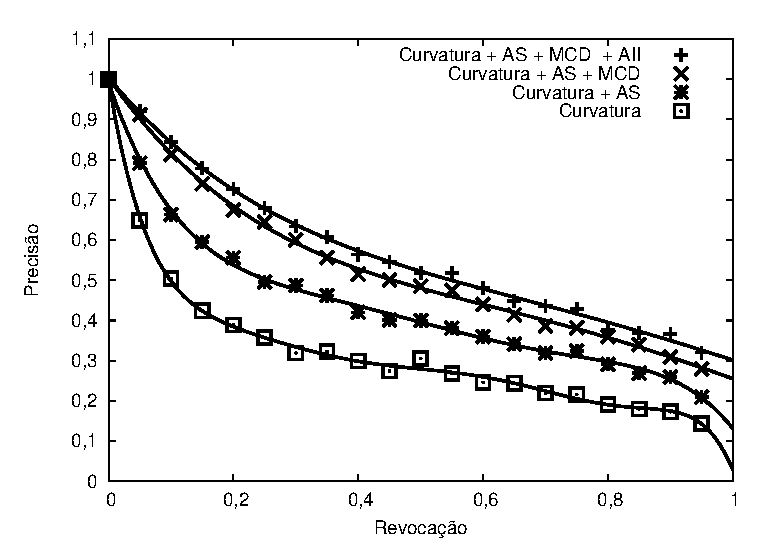
\includegraphics[width=0.75\textwidth]{graph1.eps}
\end{figure}


\section{\emph{Gap semântico}}
Uma questão importante nos sistemas \emph{CBIR} é que, embora os usuários busquem por imagens similares do ponto de vista semântico, o sistema provê os resultados com base na similaridade da informação extraída do conteúdo visual das imagens. A disparidade existente entre esses aspectos (semântica e conteúdo visual) é denominado de \emph{Gap} semântico.

Embora as imagens transmitam determinadas mensagens ao usuário, muito frequentemente os atributos extraídos das mesmas não conseguem representar e caracterizar essas mensagens. Diversos métodos para associar informação semântica aos atributos extraídos das imagens têm sido foco de pesquisa, como por exemplo solicitar que o usuário retro-alimente o sistema com o grau de relevância dos resultados obtidos (relevance feedback). 

\section{Base de imagens}

Um aspecto importante em \emph{CBIR} está ligado ao mecanismo de indexação empregado no acesso a informação contida na base de imagens. Em aplicações práticas, que requerem acesso a uma extensa base de dados, e aonde há interação dos usuários com o mecanismo de busca, o desempenho computacional no processo de indexação não pode ser negligenciado. Desta forma, armazenar vetores de características em um arquivo linear, com um registro para cada vetor, resulta na indexação sequencial destes elementos tornando essa abordagem inviável.

Todavia, mecanismos alternativos de indexação tradicionalmente encontrados na literatura, tais como \emph{k-d-b tree}, \emph{quad-tree} e \emph{R-tree} são considerados inadequados em \emph{CBIR} porque o desempenho destes se degrada substancialmente com o aumento da dimensionalidade dos dados. Ademais, para alcançar a eficiência computacional requerida sem degradar a qualidade das buscas, tais mecanismos devem levar em consideração a representação das características das imagens no processo de recuperação, ou seja, não só apenas \emph{como} indexar elementos na base de dados, mas também \emph{o que} indexar.

\end{comment}
